\documentclass[12pt]{article}
\usepackage{geometry}                % See geometry.pdf to learn the layout options. There are lots.
\geometry{letterpaper}                   % ... or a4paper or a5paper or ... 
%\geometry{landscape}                % Activate for for rotated page geometry
%\usepackage[parfill]{parskip}    % Activate to begin paragraphs with an empty line rather than an indent
\usepackage{graphicx}
\usepackage{amssymb}
\usepackage{epstopdf}
\usepackage{hyperref}
\DeclareGraphicsRule{.tif}{png}{.png}{`convert #1 `dirname #1`/`basename #1 .tif`.png}

\title{Problem Set 2}
\author{Samuel Factor}
\date{\today}                                           % Activate to display a given date or no date

\begin{document}
\maketitle
%\section{}
%\subsection{}

Source code can be found at \url{}. The file \texttt{polytrope.py} contains functions for the Lane-Emden equation, the polynomial approximation, and a function which numerically integrates both of the above equations and both returns and writes to a fits file an array of $\xi$, $\Theta$, $-\xi^2 \frac{d\Theta}{d\xi}$, $\frac{-3}{\xi}\frac{d\Theta}{d\xi}$. The file \texttt{plots.py} runs the model, calculates important values and generates plots. It first looks for a previously executed fits file with the same index, if it finds one it uses that data, if it doesn't it runs the model. 

\section{Part a}
For $n=2.9$ the value for the dimensionless radius is $\xi_{2.9}=6.52637$ and $(-\xi^2\frac{d\Theta}{d\xi})_{\xi_n}=2.04840$.

\section{Part b}
The central density $\rho_c [\mathrm{g~cm^{-3}}] =37.14942$, the normalization constant $A=1.33969\times10^{-11}$, the scaling factor $K=1.72089\times10^{16}$. The central pressure $P_c [\mathrm{dyne~cm^{-2}}] = 2.2237\times10^{18}$. With $\beta=0.5$ the central temperature given by equation 19.22 from KW$^2$ $T_c[\mathrm{K}]=1.45\times10^8$.

\section{Part c}
A plot of pressure $P [\mathrm{dyne~cm^{-2}}]$ vs. radius $r [\mathrm{cm}]$ is shown in figure \ref{fig:P}. A plot of density $\rho [\mathrm{g~cm^{-3}}]$ vs. radius $r [\mathrm{cm}]$ is shown in figure \ref{fig:p}.

\begin{figure}[htbp]
\begin{center}
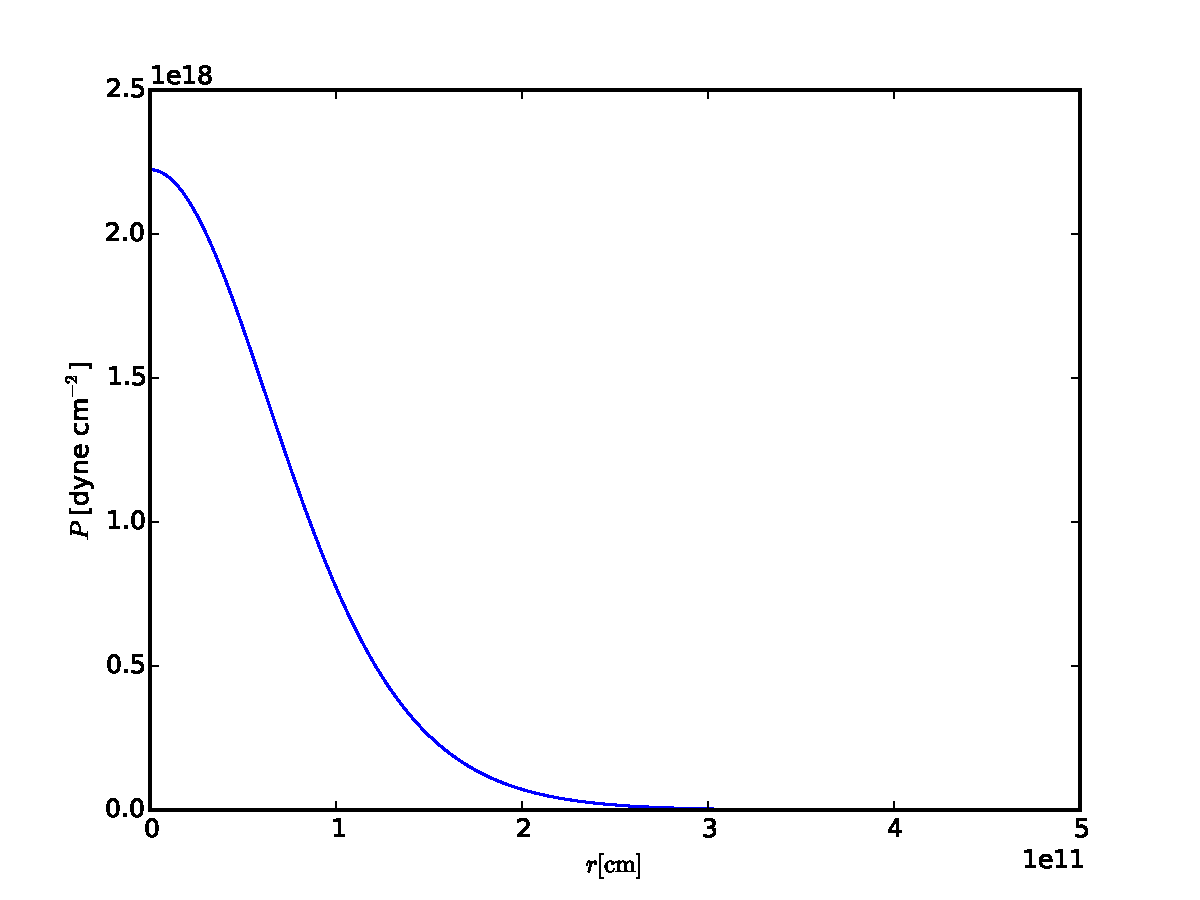
\includegraphics[width=\textwidth]{pressure2p9.pdf}
\caption{Pressure vs radius for an $n=2.9$ polytrope model of a star with $M=200M_\odot$ and $R=7R_\odot$.}
\label{fig:P}
\end{center}
\end{figure}

\begin{figure}[htbp]
\begin{center}
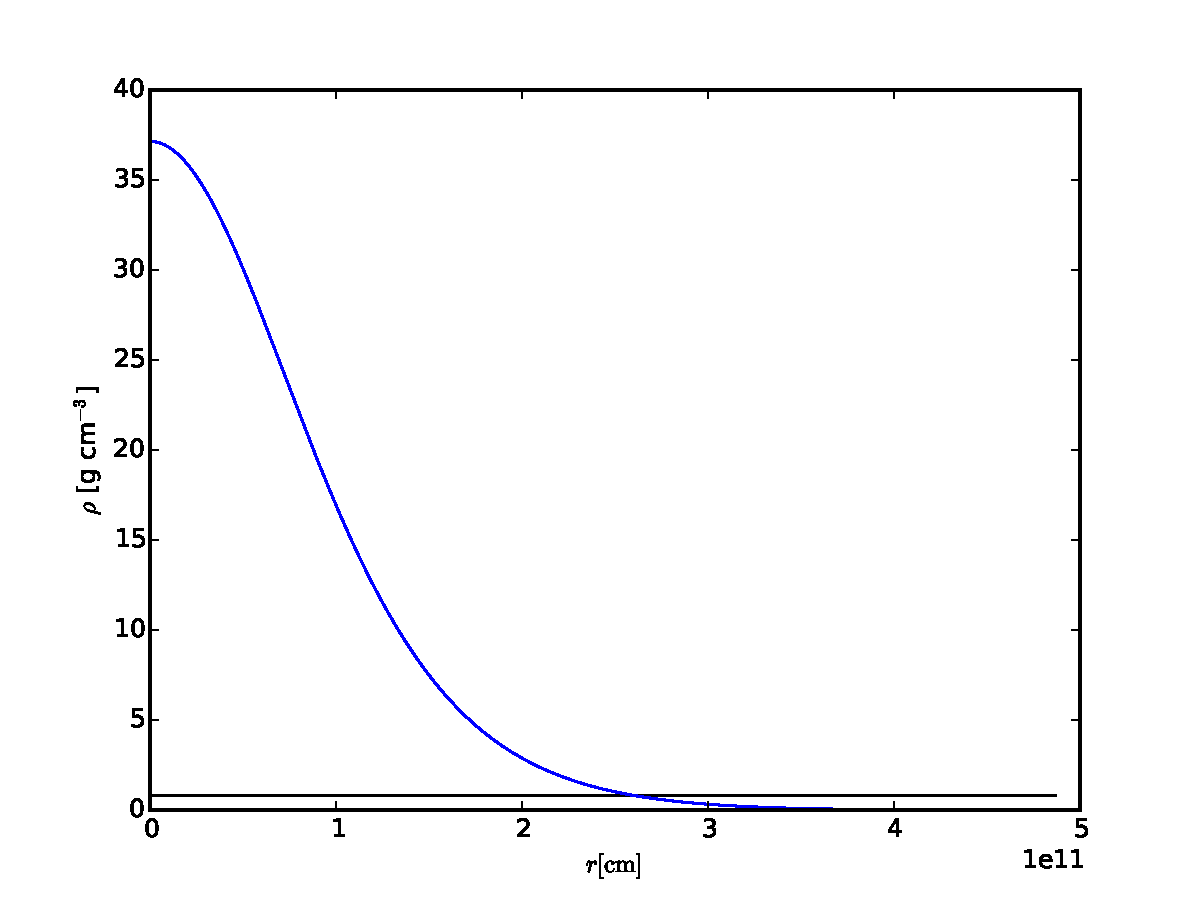
\includegraphics[width=\textwidth,keepaspectratio]{density2p9.pdf}
\caption{Density vs radius for an $n=2.9$ polytrope model of a star with $M=200M_\odot$ and $R=7R_\odot$. Black horizontal line corresponds to $\bar{\rho}$.}
\label{fig:p}
\end{center}
\end{figure}

\section{Part d}
The total gravitational potential energy of this star as given by equation 19.44 in KW$^2$ is $-3.096\times10^{52}$ ergs. As a sanity check I calculated the gravitational potential energy of a uniform density ($\rho=\bar{\rho}$) sphere and got $-1.300\times10^{52}$ which the same order of magnitude.

\end{document}  